\documentclass[12pt]{report}
\usepackage{graphicx}
\graphicspath{ {images/} }
\usepackage[english]{babel}
\usepackage{graphicx}
\begin{document}
\title{Lab4 \\ Absolute Zero}
\author{Dominic Martinez-Ta}
\date{30 April 2015}
\maketitle


\section{Purpose}
	
	To investigate how the pressure of a given quantity of gas in a fixed volume varies with
the temperature. This relationship between pressure and temperature, which is approximately
linear for low number densities and temperatures somewhat above liquefaction, is
extrapolated to zero pressure. The temperature at which this occurs is absolute zero.

\section {Materials and resources}

Data Studio, Water, Salt, Hot water, Dry Ice, Thermometers, Pressure meter. Love.

\section{Procedure}
	\begin{enumerate}
		\item  Start with the bulb submerged hot water. Be careful not to open the bulb during the experiment.
		\item When the temperature on the digits display stabilizes, log the data point.
		\item Cool the system by adding cold water, taking new data points when appropriate.
		\item Stir the water with the bulb using a vertical motion, but do not expose the top of the bulb to the air. It must always remain submerged.
		\item  If the water container becomes too full, remove a small amount of the water.
	\end{enumerate}
	Fit this data and record your results. Be sure to include error analysis and error bars in your fit.

	To obtain a lower temperature point, we will cool salt water using dry ice.
	\begin{enumerate}
		\item Make a 7 m solution of salt water. You can lookup how to do this. Do not just pour in lots of salt or there will not be enough for the other groups. Compute the correct amount of salt to add to make the 7 m solution.
		\item Make sure the final total amount of solution you make will not overflow out of the container. The liquid level will rise when you introduce the bulb and dry ice. Be sure to leave enough room for this. You will need to stir for 5 min to 10 min to dissolve the salt.
		\item If you cool the solution to 0 °C using ice you will dilute the solution. Either determine how to compensate for this to maintain the 7 m concentration, or only use the dry ice to cool the solution.
		\item Start with the bulb fully submerged. Add dry ice to cool the solution until it reaches the minimum temperature of a salt water and dry ice bath. Do not add so much that the solution freezes. Continuously agitate the solution with the bulb to prevent this.
	\end{enumerate}
\section{Data Analysis}
	
	We were able to see that as we decreased the temperature, as did the pressure of the entire system. This means that everything  we saw was according to the Laws of of Thermodynamics. With our measurements, we saw that the pressure of the gas within the sphere was proportional to the temperature of the system. We also saw that we had a total slope of -0.4733. Thus showing us how slowly our graph of absolute zero, went to zero. (Of course, we couldn't measure that with such a simple experiment.)

\section{Questions}
\begin{enumerate}
	  \item Observe and document in your lab notebook all equipment operation and possible systematics that could effect your measurement.
 	 \begin{enumerate}
  		  \item Did you notice that the T and P sensors are sometimes changing at different rates?
  		  \item Did you see systematic drifting of (T , P) pairs? What could cause that?
 		   \item How does the data you have taken and chosen to fit effect the accuracy of your fit value of T$_{\circ}$.
 		   \item Could the T and P sensors be in a different location inside the sphere?
   		  \item Why do the directions say the sphere needs to be fully submerged at all times while taking data?
   		  \item What about water vapor inside the sphere?
  	\end{enumerate}
 
	\item  Estimate how accurately you need to obtain data in order to reach your goal, and assess what is needed to get that accuracy.
	\begin{enumerate}
		\item How accuately would you have to measure two data points at -2$^{\circ}$C to -60$^{\circ}$C to measure T$_{\circ}$ with a precision of $\pm$1$^{\circ}$.
		\item What about N points assuming normal (Gaussian) distribution of experimental measurement error?
		\item Calculate the contribution of  $ \chi ^2$ due to the error bar per measurement.
		\item Why does the confidence in the fit scale as $\sqrt{\frac{\chi ^2}{N}}$ Where N is number of points.
	\end{enumerate}


	\item Consider physical corrections to the data and analysis
	 \begin{enumerate}
		\item Look up and calculate the effect of water vapor and thermal expansion for your apparatus.
		\item Calculate the size of these effects and therefore the accuracy of fit, and thus the number of data points you need to obtain to correct for these effects.
	\end{enumerate}

	\item Data and analysis and curve fitting
	\begin{enumerate}
		\item Find the fit function you will use and the number of free variables needed.
		\item Review standard deviation, root-mean-square error (RMSE), variance, quality of fit etc.
	\end{enumerate}

\end{enumerate}
\section{Answers}
	\begin{enumerate}
		\item 
		\begin{enumerate}
			\item I did notice that T and P sensors were sometimes changing at different rates. This was because the temperature was more controllable than the pressure. Meaning that temperature was being more affected by the outside variables, while the temperature inside the sphere would be changing at a different rate. So therefore, the pressure inside would change at a different rate as a result. This means that T$_{outside}$ $>$ T$_{inside}$
			\item The systematic drifting of the T and P pairs would be because of the inverse relationship they have towards one another. But as the entire system reaches an equilibium of temperature, the pressure would still be changing inside the sphere because the temperature within it has not equalized yet. Thus, as our system cools down, the pressure being measured will not be measured correctly accordingly to the T$_{outside}$
			\item The Data I took and chose to fit effects the accuracy of my fit value or T$_{\circ}$ by throwing the overall slope of the linear fit off. The slope should be an approximate, but as our values change sporadically, our linear fit becomes harder to approximate. 
			\item The T and P sensours \emph{could} be in a different located inside the sphere, but it would be difficult to know. To figure this out, we would have had to change the temperature rapidly on different parts of the sphere, to see which part measured the change the quickest. That would be the easiest way to know where the sensors are located. 
			\item The directions tell us that the sphere needs to be fully submerged at all times while taking data, because we would have huge changes (or jumps) in temperature and or pressure. This as a result, would skew our data and give us a very large errors.
			\item The water vapor inside the sphere is what is measuring the temperature, as the pressure is being measured by within the sphere. Thus, this is why the temperature would be measuered at a different speed than the temperature. 
		\end{enumerate}
		\item
		\begin{enumerate}
			\item To accurately measure two data points in between -2$^{\circ}$C and-60 $^{\circ}$C, with an error no more than $\pm 1^{\circ}$, we would basically need to have a slope of $\frac{-2 + 60}{t_1 - t_2}$ and a y intercept of -2$^{\circ}$C. This would give us an error of about $\pm 1^{\circ}$ or less. Our errors were less than $\pm$0.023 according to our graphs so we did just that.
			\item For N points, we would need not need to be very accurate in measuring data until our points become fewer and fewer. Thus the larger the N, the more accurate we would have to be.
			\item The contribution of  $\chi ^2$ due to the error bar per measurement was 2.65
			\item The confidence int he fit scale as $\sqrt{\frac{\chi ^2}{N}}$ (I DO NOT UNDERSTAND THIS QUESTION, SO I AM ANSWERING TO THE BEST OF MY ABILITIES) SO this is the Root MSE which is 1.63.
		\end{enumerate}
		\item
		\begin{enumerate}
			\item The effect of water vapor and thermal expansion of our apparatus would be around 0.03 \%  which is approximate to our error of the total data graph.
			\item We would have needed aroudn 15 data points to correct for the accuracy of fit and size of the effects. The error was too little to really worry about. It did not change the experiment very much.

			
		\end{enumerate}
\end{enumerate}
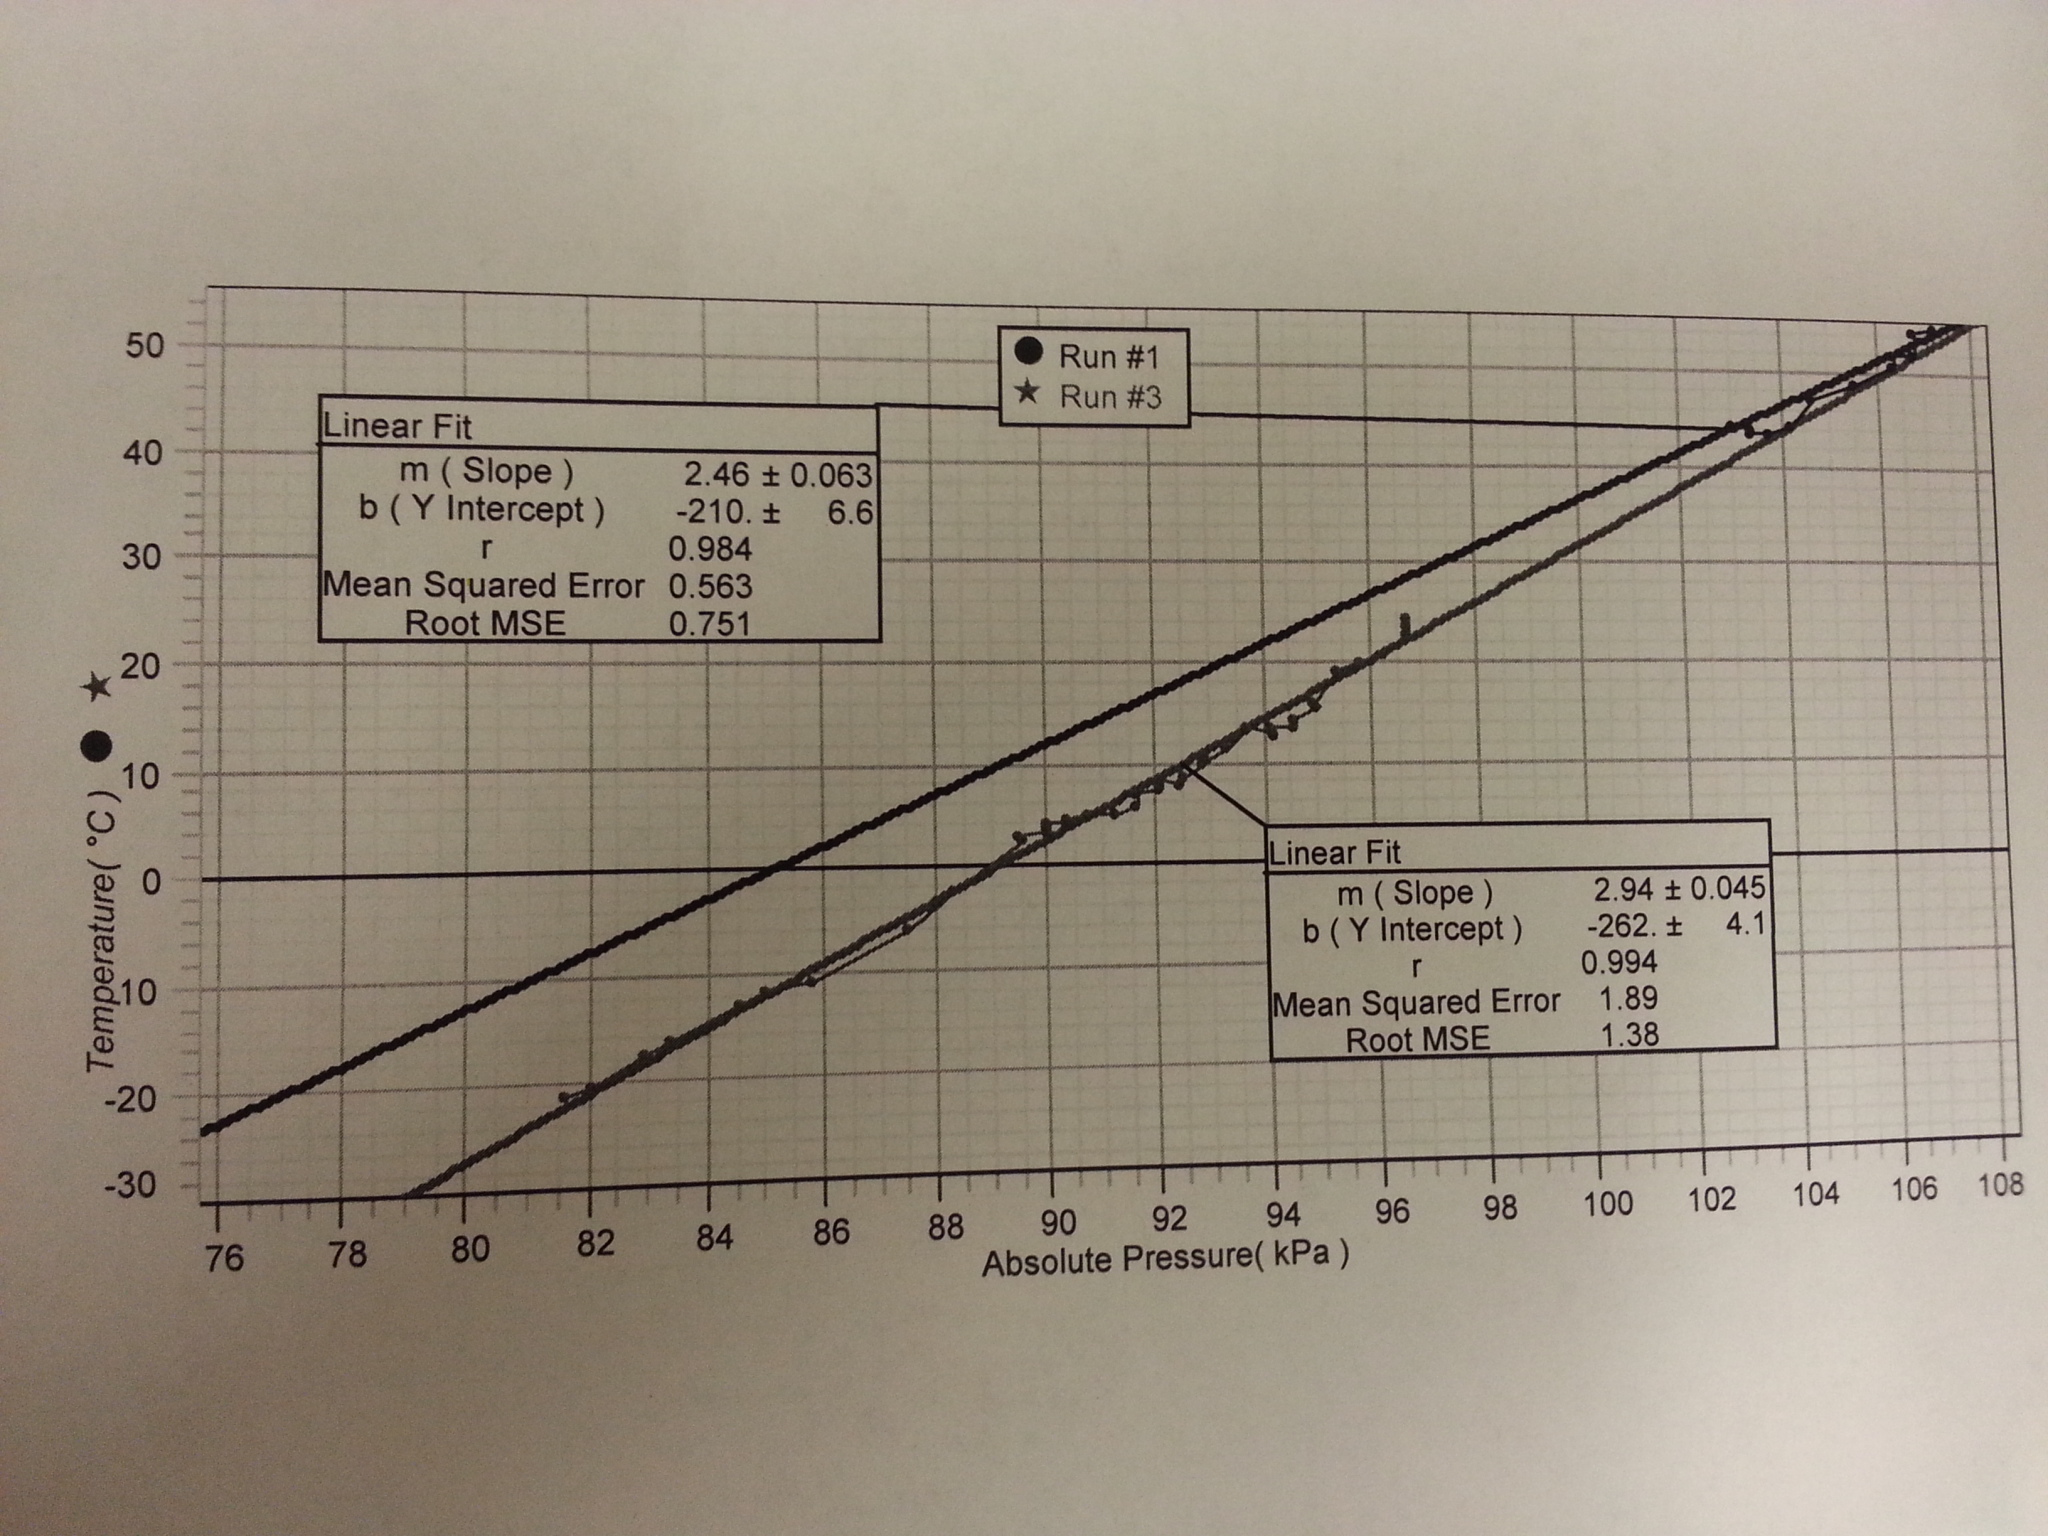
\includegraphics[scale=0.2]{both_graphs}
Above, is the image of both of my measurements as graphs from both parts of the experiment.\\
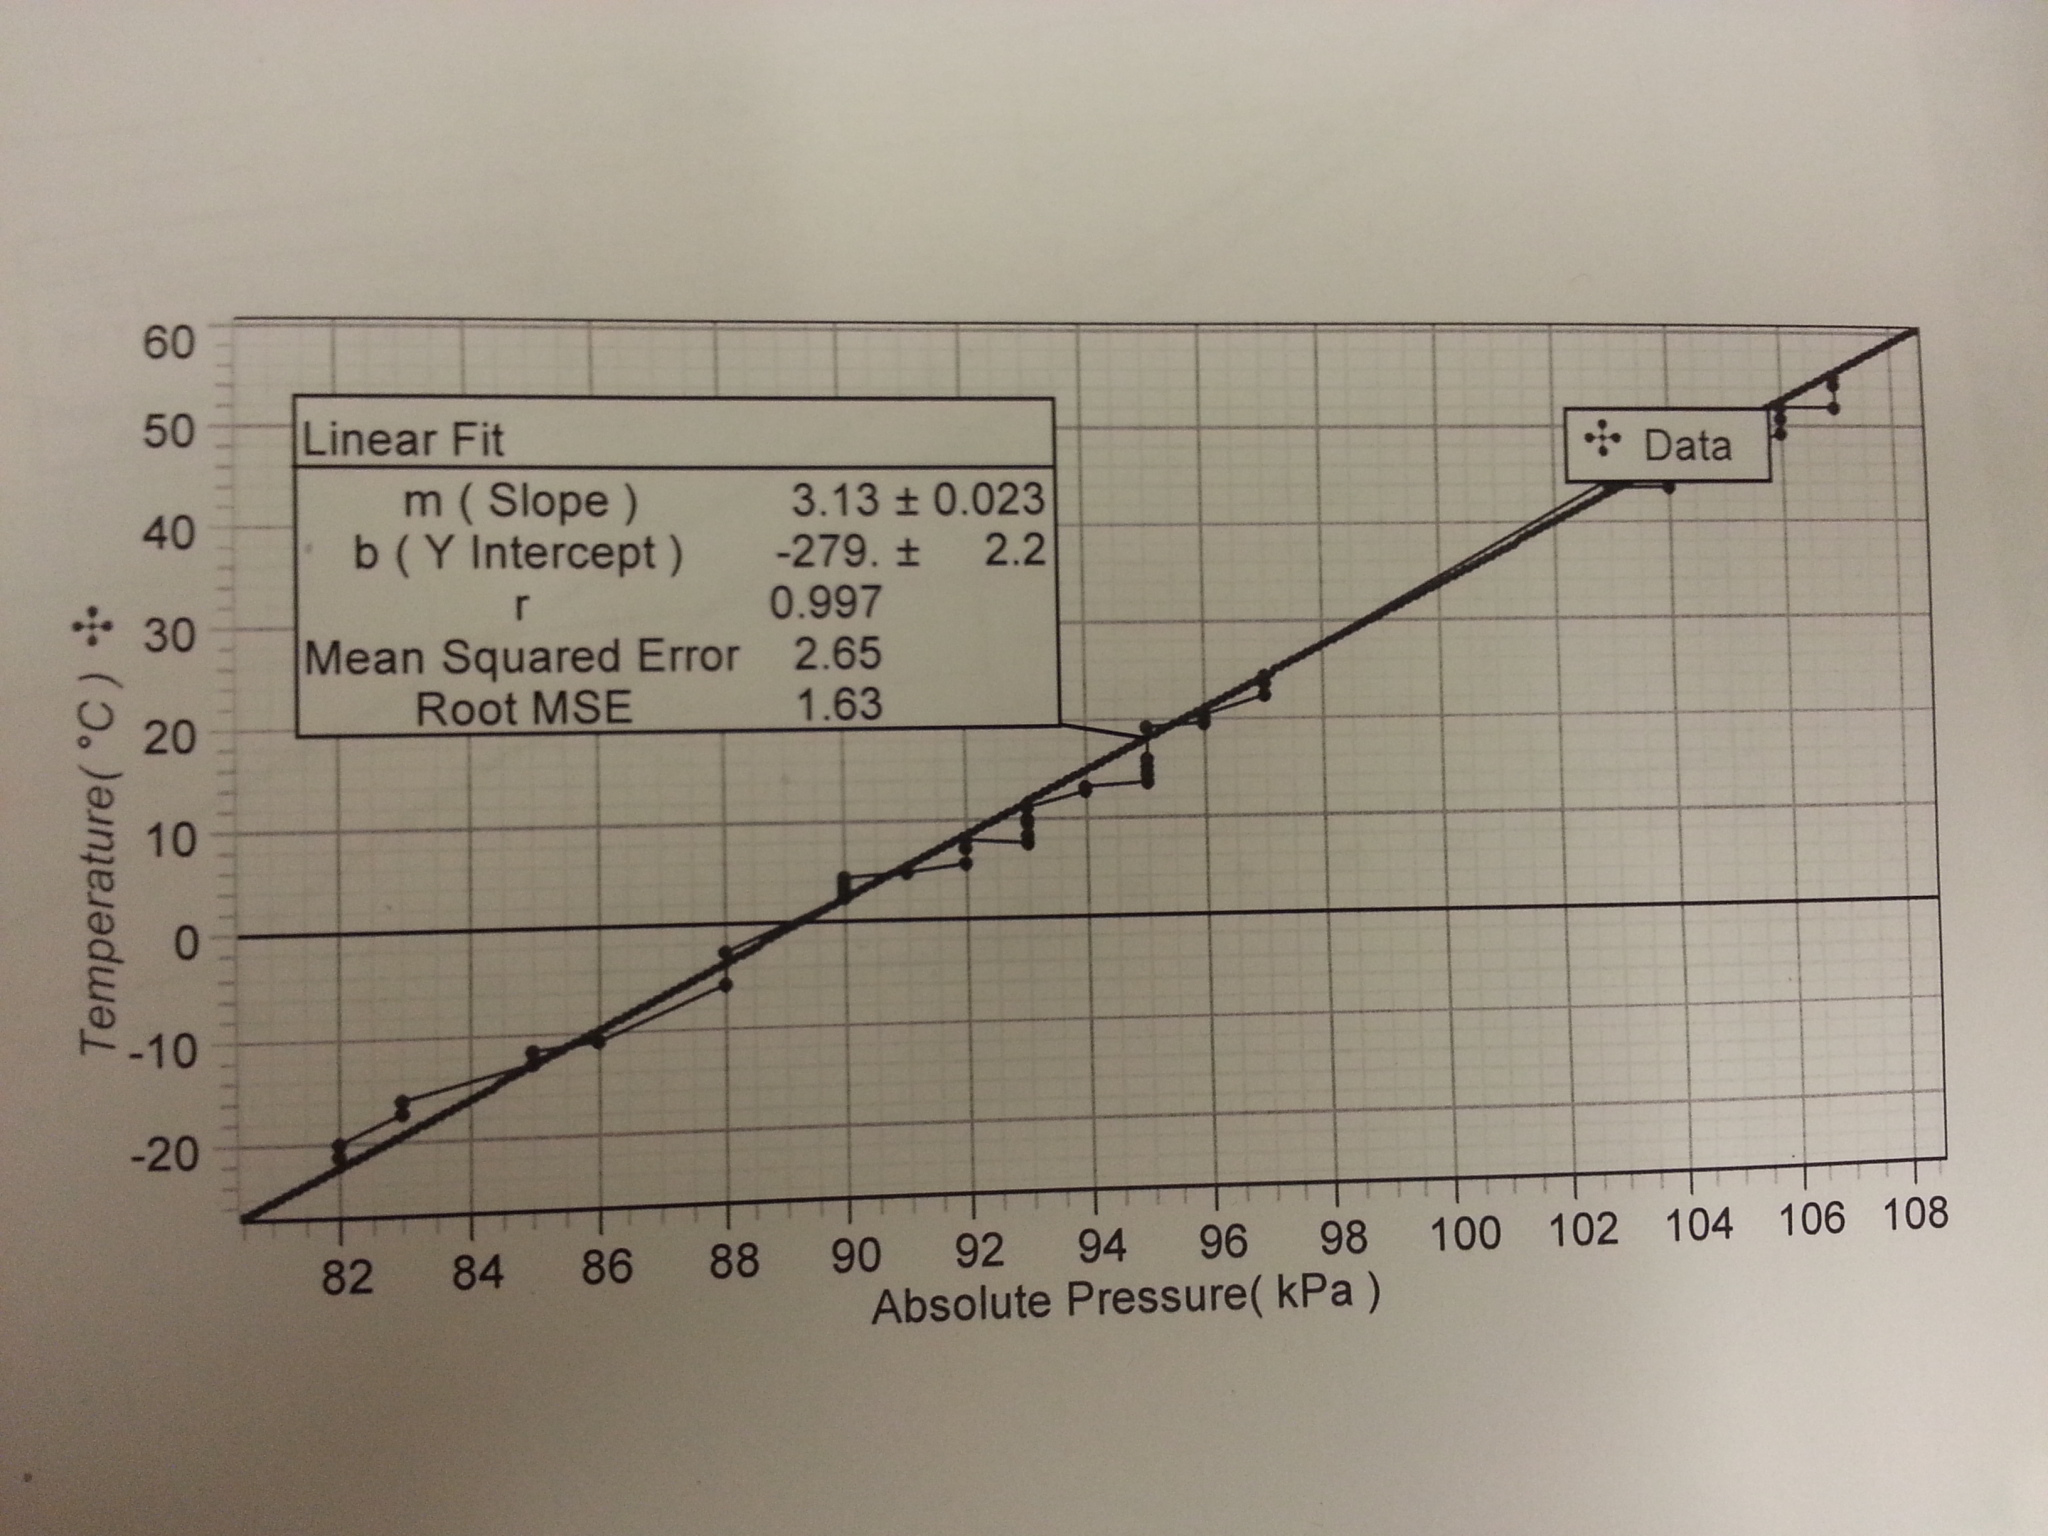
\includegraphics[scale=0.2]{OverallGraphs}
Above is the image of the overall graph of both parts of the experiment.
Both of these pictures are for number 4.
\end{document}